\documentclass[tikz,crop,convert={density=200,outext=.png},border=0.4cm]{standalone}

\usepackage{pgfplots}
\usepackage{amsmath}
\usetikzlibrary{arrows.meta}
\usepackage{physics}
\usepackage{xcolor}
\definecolor{exp_1}{RGB}{0,68,27}
\pgfplotsset{compat=newest,
    %width=6cm,
    %height=3cm,
    scale only axis=true,
    max space between ticks=25pt,
    try min ticks=5,
    every axis/.style={
        axis y line=middle,
        axis x line=middle,
        axis line style={thick,->,>=latex, shorten >=-.3cm}
    },
    every axis plot/.append style={thick},
    tick style={black, thick},
}
\tikzset{
    semithick/.style={line width=0.8pt},
}
\usepgfplotslibrary{groupplots}
\usepgfplotslibrary{dateplot}
% Document begins
\begin{document}
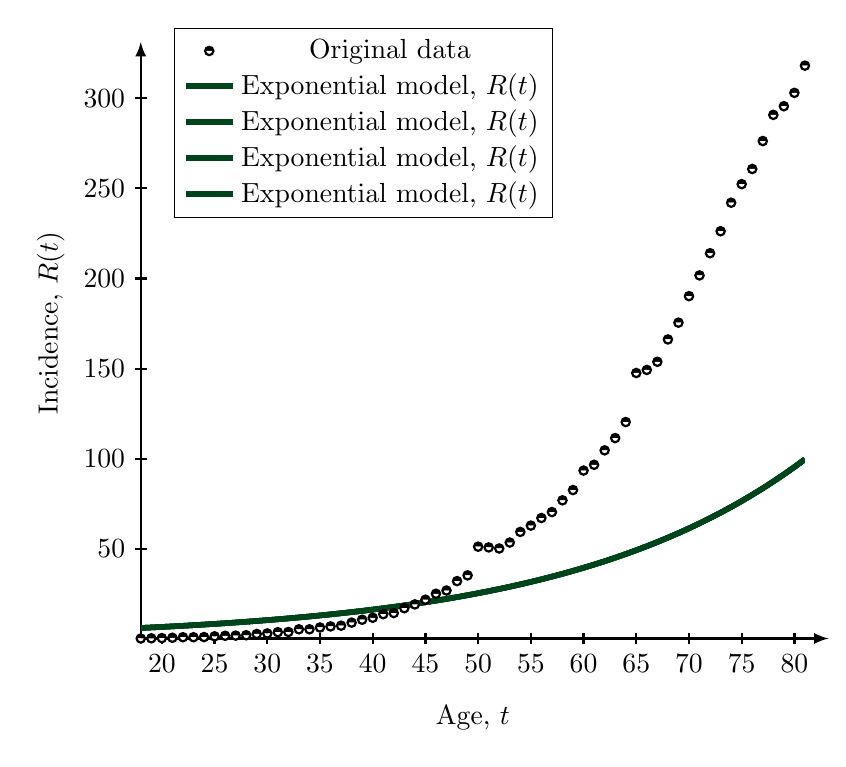
\begin{tikzpicture}
  % The axis of the plot
\begin{axis}[
    %title={Model: $\dv{y}{t}=\frac{2y}{t}$ with solution $y(t)=C_1t^2$\\Symmetry: $\Gamma_{\epsilon}=(t,y)\mapsto\left(\exp\left(\epsilon\right)t,\exp\left(-\epsilon\right)y\right)$},
    title style = {align=left},
    xlabel={Age, $t$},
    ylabel={Incidence, $R(t)$},
    x label style={at={(axis description cs:0.5,-0.1)},anchor=north},
    y label style={at={(axis description cs:-0.1,0.55)},rotate=90,anchor=south},    
    %xmin=-27, xmax=5,
    %ymin=-20, ymax=20,
    %xtick={-30,-27,...,9},
    %ytick={-15,-10,...,15},
    legend style={at={(axis description cs:0.05,0.9)},anchor=west},    
    %legend pos=north west,
    %ymajorgrids=true,
    grid style=dashed,
]
% Plot the data
\addplot[
only marks, mark=halfcircle*,mark size=1.5pt,color=black,
]
coordinates {%
(18.0,0.4)
(19.0,0.5)
(20.0,0.6)
(21.0,0.8)
(22.0,1.1)
(23.0,1.1)
(24.0,1.2)
(25.0,1.6)
(26.0,1.9)
(27.0,2.0)
(28.0,2.2)
(29.0,2.9)
(30.0,3.2)
(31.0,3.8999999999999995)
(32.0,4.0)
(33.0,5.5)
(34.0,5.5)
(35.0,6.499999999999999)
(36.0,7.1000000000000005)
(37.0,7.499999999999999)
(38.0,9.2)
(39.0,10.8)
(40.0,11.9)
(41.0,13.9)
(42.0,14.5)
(43.0,17.2)
(44.0,19.299999999999997)
(45.0,21.9)
(46.0,25.199999999999996)
(47.0,27.0)
(48.0,32.2)
(49.0,35.4)
(50.0,51.300000000000004)
(51.0,50.9)
(52.0,50.29999999999999)
(53.0,53.60000000000001)
(54.0,59.50000000000001)
(55.0,62.99999999999999)
(56.0,67.19999999999999)
(57.0,70.5)
(58.0,77.00000000000001)
(59.0,82.69999999999997)
(60.0,93.50000000000001)
(61.0,96.69999999999996)
(62.0,104.69999999999999)
(63.0,111.5)
(64.0,120.39999999999995)
(65.0,147.59999999999997)
(66.0,149.29999999999995)
(67.0,153.80000000000004)
(68.0,166.20000000000005)
(69.0,175.50000000000009)
(70.0,190.2)
(71.0,201.70000000000007)
(72.0,213.99999999999994)
(73.0,226.20000000000007)
(74.0,242.00000000000009)
(75.0,252.3000000000001)
(76.0,260.70000000000005)
(77.0,276.20000000000005)
(78.0,290.7000000000001)
(79.0,295.50000000000006)
(80.0,302.8999999999999)
(81.0,318.0)
};
\addlegendentry{Original data}

% Plot the model
\addplot[
color=exp_1,line width=2pt,
]
coordinates {%
(18.0,6.238595703991077)
(19.0,6.519222429953524)
(20.0,6.812472406894396)
(21.0,7.11891345836905)
(22.0,7.439138949973528)
(23.0,7.773768938285679)
(24.0,8.12345137148841)
(25.0,8.488863343999714)
(26.0,8.87071240753901)
(27.0,9.269737941168252)
(28.0,9.686712582960755)
(29.0,10.12244372606985)
(30.0,10.57777508209422)
(31.0,11.053588314767126)
(32.0,11.550804747132732)
(33.0,12.070387145515383)
(34.0,12.613341583735862)
(35.0,13.180719391184633)
(36.0,13.773619188523893)
(37.0,14.393189014960354)
(38.0,15.040628551207753)
(39.0,15.71719144244344)
(40.0,16.424187725757044)
(41.0,17.16298636679146)
(42.0,17.935017910488007)
(43.0,18.741777251068168)
(44.0,19.584826526615885)
(45.0,20.46579814386472)
(46.0,21.38639793904731)
(47.0,22.34840848092701)
(48.0,23.353692522407986)
(49.0,24.404196607406526)
(50.0,25.50195483996823)
(51.0,26.649092822928765)
(52.0,27.847831773744815)
(53.0,29.100492825465096)
(54.0,30.409501521168767)
(55.0,31.777392510574668)
(56.0,33.2068144579147)
(57.0,34.70053517057534)
(58.0,36.26144695843707)
(59.0,37.89257223428995)
(60.0,39.597069366168796)
(61.0,41.37823879294011)
(62.0,43.23952941498293)
(63.0,45.184545272336976)
(64.0,47.21705252325022)
(65.0,49.34098673663733)
(66.0,51.56046051257077)
(67.0,53.8797714455588)
(68.0,56.303410446031194)
(69.0,58.83607043614426)
(70.0,61.48265543674435)
(71.0,64.24829006308393)
(72.0,67.13832944767721)
(73.0,70.15836960950992)
(74.0,73.31425828967947)
(75.0,76.6121062744489)
(76.0,80.0582992276373)
(77.0,83.65951005526014)
(78.0,87.42271182635915)
(79.0,91.35519127504264)
(80.0,95.46456290987823)
(81.0,99.7587837579605)
};
\addlegendentry{Exponential model, $R(t)$}
\addplot[
color=exp_1,line width=2pt,
]
coordinates {%
(18.0,6.238595703991077)
(19.0,6.519222429953524)
(20.0,6.812472406894396)
(21.0,7.11891345836905)
(22.0,7.439138949973528)
(23.0,7.773768938285679)
(24.0,8.12345137148841)
(25.0,8.488863343999714)
(26.0,8.87071240753901)
(27.0,9.269737941168252)
(28.0,9.686712582960755)
(29.0,10.12244372606985)
(30.0,10.57777508209422)
(31.0,11.053588314767126)
(32.0,11.550804747132732)
(33.0,12.070387145515383)
(34.0,12.613341583735862)
(35.0,13.180719391184633)
(36.0,13.773619188523893)
(37.0,14.393189014960354)
(38.0,15.040628551207753)
(39.0,15.71719144244344)
(40.0,16.424187725757044)
(41.0,17.16298636679146)
(42.0,17.935017910488007)
(43.0,18.741777251068168)
(44.0,19.584826526615885)
(45.0,20.46579814386472)
(46.0,21.38639793904731)
(47.0,22.34840848092701)
(48.0,23.353692522407986)
(49.0,24.404196607406526)
(50.0,25.50195483996823)
(51.0,26.649092822928765)
(52.0,27.847831773744815)
(53.0,29.100492825465096)
(54.0,30.409501521168767)
(55.0,31.777392510574668)
(56.0,33.2068144579147)
(57.0,34.70053517057534)
(58.0,36.26144695843707)
(59.0,37.89257223428995)
(60.0,39.597069366168796)
(61.0,41.37823879294011)
(62.0,43.23952941498293)
(63.0,45.184545272336976)
(64.0,47.21705252325022)
(65.0,49.34098673663733)
(66.0,51.56046051257077)
(67.0,53.8797714455588)
(68.0,56.303410446031194)
(69.0,58.83607043614426)
(70.0,61.48265543674435)
(71.0,64.24829006308393)
(72.0,67.13832944767721)
(73.0,70.15836960950992)
(74.0,73.31425828967947)
(75.0,76.6121062744489)
(76.0,80.0582992276373)
(77.0,83.65951005526014)
(78.0,87.42271182635915)
(79.0,91.35519127504264)
(80.0,95.46456290987823)
(81.0,99.7587837579605)
};
\addlegendentry{Exponential model, $R(t)$}
\addplot[
color=exp_1,line width=2pt,
]
coordinates {%
(18.0,6.238595703991077)
(19.0,6.519222429953524)
(20.0,6.812472406894396)
(21.0,7.11891345836905)
(22.0,7.439138949973528)
(23.0,7.773768938285679)
(24.0,8.12345137148841)
(25.0,8.488863343999714)
(26.0,8.87071240753901)
(27.0,9.269737941168252)
(28.0,9.686712582960755)
(29.0,10.12244372606985)
(30.0,10.57777508209422)
(31.0,11.053588314767126)
(32.0,11.550804747132732)
(33.0,12.070387145515383)
(34.0,12.613341583735862)
(35.0,13.180719391184633)
(36.0,13.773619188523893)
(37.0,14.393189014960354)
(38.0,15.040628551207753)
(39.0,15.71719144244344)
(40.0,16.424187725757044)
(41.0,17.16298636679146)
(42.0,17.935017910488007)
(43.0,18.741777251068168)
(44.0,19.584826526615885)
(45.0,20.46579814386472)
(46.0,21.38639793904731)
(47.0,22.34840848092701)
(48.0,23.353692522407986)
(49.0,24.404196607406526)
(50.0,25.50195483996823)
(51.0,26.649092822928765)
(52.0,27.847831773744815)
(53.0,29.100492825465096)
(54.0,30.409501521168767)
(55.0,31.777392510574668)
(56.0,33.2068144579147)
(57.0,34.70053517057534)
(58.0,36.26144695843707)
(59.0,37.89257223428995)
(60.0,39.597069366168796)
(61.0,41.37823879294011)
(62.0,43.23952941498293)
(63.0,45.184545272336976)
(64.0,47.21705252325022)
(65.0,49.34098673663733)
(66.0,51.56046051257077)
(67.0,53.8797714455588)
(68.0,56.303410446031194)
(69.0,58.83607043614426)
(70.0,61.48265543674435)
(71.0,64.24829006308393)
(72.0,67.13832944767721)
(73.0,70.15836960950992)
(74.0,73.31425828967947)
(75.0,76.6121062744489)
(76.0,80.0582992276373)
(77.0,83.65951005526014)
(78.0,87.42271182635915)
(79.0,91.35519127504264)
(80.0,95.46456290987823)
(81.0,99.7587837579605)
};
\addlegendentry{Exponential model, $R(t)$}
\addplot[
color=exp_1,line width=2pt,
]
coordinates {%
(18.0,6.238595703991077)
(19.0,6.519222429953524)
(20.0,6.812472406894396)
(21.0,7.11891345836905)
(22.0,7.439138949973528)
(23.0,7.773768938285679)
(24.0,8.12345137148841)
(25.0,8.488863343999714)
(26.0,8.87071240753901)
(27.0,9.269737941168252)
(28.0,9.686712582960755)
(29.0,10.12244372606985)
(30.0,10.57777508209422)
(31.0,11.053588314767126)
(32.0,11.550804747132732)
(33.0,12.070387145515383)
(34.0,12.613341583735862)
(35.0,13.180719391184633)
(36.0,13.773619188523893)
(37.0,14.393189014960354)
(38.0,15.040628551207753)
(39.0,15.71719144244344)
(40.0,16.424187725757044)
(41.0,17.16298636679146)
(42.0,17.935017910488007)
(43.0,18.741777251068168)
(44.0,19.584826526615885)
(45.0,20.46579814386472)
(46.0,21.38639793904731)
(47.0,22.34840848092701)
(48.0,23.353692522407986)
(49.0,24.404196607406526)
(50.0,25.50195483996823)
(51.0,26.649092822928765)
(52.0,27.847831773744815)
(53.0,29.100492825465096)
(54.0,30.409501521168767)
(55.0,31.777392510574668)
(56.0,33.2068144579147)
(57.0,34.70053517057534)
(58.0,36.26144695843707)
(59.0,37.89257223428995)
(60.0,39.597069366168796)
(61.0,41.37823879294011)
(62.0,43.23952941498293)
(63.0,45.184545272336976)
(64.0,47.21705252325022)
(65.0,49.34098673663733)
(66.0,51.56046051257077)
(67.0,53.8797714455588)
(68.0,56.303410446031194)
(69.0,58.83607043614426)
(70.0,61.48265543674435)
(71.0,64.24829006308393)
(72.0,67.13832944767721)
(73.0,70.15836960950992)
(74.0,73.31425828967947)
(75.0,76.6121062744489)
(76.0,80.0582992276373)
(77.0,83.65951005526014)
(78.0,87.42271182635915)
(79.0,91.35519127504264)
(80.0,95.46456290987823)
(81.0,99.7587837579605)
};
\addlegendentry{Exponential model, $R(t)$}

\end{axis}
\end{tikzpicture}

\end{document}
